\section{Experiment Details and Evidence Boundaries}
\label{sec:appendix-experiments}

This appendix records the technical details behind Section~\ref{sec:main-experiments}. The tables in this appendix report the original runs of each experiment. Fig.~\ref{fig:experiments} and its detailed versions, Figs.~\ref{fig:appendix-synthetic} and~\ref{fig:appendix-realdata}, also include data sets added later with seeds fixed in advance, for $100$ data sets per synthetic setting, $100$ Twins replicates, and $88$ IHDP replicates in total, so their MAE values differ from the tables. The tables report PROBE with the blocks given; the figures report it with the blocks it finds from $W$, except in the image settings (Appendix~\ref{sec:appendix-block-discovery}).

\subsection{Shared structural family}

All four confirmations share one structure. Let $U$ be the hidden confounder, $I$ a treatment-only cause, $C$ an observed confounder, and let $\eta$, $\epsilon_0,\ldots,\epsilon_4$ and $\varepsilon_Y$ be independent standard normal noises. The informative coordinates, which no learner sees by name, are
\(X_1=U+2\eta,\qquad M_j=U+0.85\,\epsilon_j\ (j=0,\ldots,3),\qquad M_4=U-3.0\,I+0.85\,\epsilon_4.\)
Treatment and outcome follow
\(P(A=1\mid U,I,C,X_1)=0.1+0.8\,\Phi(1.5U+2.0I+0.2X_1+0.3C),\qquad Y(a)=a-2.5U+0.2X_1-0.5C+0.3\varepsilon_Y,\)
so the average treatment effect is $\tau=1$. The observed covariate $X$ carries $X_1$ and $C$. Blocks $W_1,W_2,W_3$ carry $M_1,M_2,M_3$, block $W_4$ carries the contaminated $M_4$, and block $W_5$ carries $M_0$ together with $I$. Each observed vector is a fixed random rotation of its informative coordinates stacked on pure noise coordinates with standard deviation $0.5$, so no observed coordinate is a named quantity. Placing $C$ inside $X$, which always enters the representation, prevents a representation from dropping an outcome-relevant coordinate in order to balance.

The three numeric settings differ only in how many noise coordinates hide the informative ones. SCM-1 gives $X$ two coordinates and the five blocks $(1,1,1,1,2)$ coordinates, for $8$ in total. SCM-2 gives $X$ eight and each block sixteen, for $88$. SCM-3 gives $X$ thirty-two and each block $256$, for $1{,}312$. Because the coefficients are shared, the population values and the census of balanceable splits are the same objects across the three.

In the population of this family, seven of the thirty candidate splits admit exact balance and target $\tau$, namely those built from the clean blocks $W_1,W_2,W_3$; the split that holds out $W_4$ also admits balance and targets a different value; the seven splits that mix $W_4$ with a clean block admit no balance; every split containing $W_5$ admits no balance at all. This is the census the screen is measured against when we report true and false positive rates.

\subsection{Image rendering}
\label{sec:appendix-image-rendering}

SCM-4 keeps the structure above and changes only what the learner receives in place of the six observed proxy coordinates. Each coordinate is recorded to $15$ equally spaced levels on $[-3\sigma,3\sigma]$, where $\sigma$ is its exact population standard deviation, and is then shown as one original $64\times64$ RGB Shapes3D image whose orientation factor equals that level. Every other generative factor of the image is drawn uniformly and independently, so the image carries the recorded level and nothing else about the unit. Blocks $W_1$ to $W_4$ contribute one image each and $W_5$ contributes two, giving six images per unit.

A frozen reader maps one image back to one number. It is a convolutional network trained with orientation labels on an image bank disjoint from every image used in the causal data, and it is never refitted during the experiment. Across the $14{,}400{,}000$ reads of all $100$ data sets it produced no level error, so SCM-4 measures the pipeline under an image proxy and not the discovery of a representation from raw pixels. The pixel CNN comparator in Section~\ref{sec:main-experiments} is a convolutional network fitted on all six images without holding out a block and without the balance screen.

Two of the twenty SCM-4 data sets reached the wall-clock cap for that comparator while three tasks shared one GPU, and the sealed summary therefore recorded FAIL on the completeness gate and on the comparison that depends on it. The two comparator runs were repeated alone under the sealed configuration and the sealed seeds, and nothing else was rerun or changed. The sealed summary and the amended summary are both retained; the amended one passes all $13$ gates.

\subsection{Search family, screen, and aggregation}

The search ranges over the thirty nonempty proper subsets of the five blocks, or over the $2^J-2$ subsets of the $J$ blocks found from $W$ (Appendix~\ref{sec:appendix-block-discovery}). For a split $S$ the representation is $Z_S=(X,Bv_{-S})$, where $v_{-S}$ stacks the preprocessed kept blocks and $B$ has rank $k=2$. Preprocessing standardises $X$ and reduces any block with more than two coordinates to its principal directions above the Marchenko--Pastur edge, at most four, fitted on the representation fold alone. The family is therefore linear in the observed coordinates and role-blind: it receives no label identifying a block, but it is not an unrestricted neural encoder.

Each data set is split into four folds of nearly equal size, $6{,}000$ rows each here, rotated so that every fold serves once as representation, screen, nuisance, and evaluation sample. The critics are bounded probit models with link $0.1+0.8\Phi$ and ridge $10^{-4}$; the augmented critic nests the base one, and the lifted base is a candidate whenever the augmented fit cannot improve on it. The screen statistic is the held-out Brier risk difference on the screen fold, refitted there rather than reused from the search and cross-fitted by row parity. A split is retained when $\max(\mathrm{gap},0)+z\,\mathrm{SE}$ falls below the threshold and every base-critic prediction on that fold lies in $[0.05,0.95]$, with $z=\Phi^{-1}(1-0.05/30)\approx 2.935$ for the thirty simultaneous decisions. The thresholds are $1.5$, $1.8$, $1.6$ and $1.7$ times $10^{-3}$ for SCM-1 to SCM-4, each fixed on development data before the confirmation seeds were generated. Retained splits are grouped by single linkage at twice a common radius, and the reported estimate is the median of the largest agreeing group, with no estimate returned when two groups tie for largest. Relative to Algorithm~\ref{alg:probe-search}, this implementation searches all $30$ splits ($m=T$), adds a separate screen fold to the three samples, retains a split only if it passes the screen in all four rotations, averages its estimate over the rotations, and sets the linking radius $\rho$ from the data by a Gaussian multiplier bootstrap. Appendix~\ref{sec:appendix-implementation} states every one of these choices in full.

\subsection{Honest learning and evaluation}

The four folds of a data set carry four separate jobs, and every rotation assigns each fold to each job once. The representation and its search critics use the representation fold. The screen refits fresh critics on the screen fold, so no statistic that decides retention was fitted on the rows that produced the representation. Propensity and outcome nuisance functions use the nuisance fold, and the AIPW score uses the evaluation fold. Preprocessing parameters are estimated only from the fold that is training at that step, and the four rotations are averaged.

For a fixed representation, the base critic predicts $A$ from $Z$, and the augmented critic predicts $A$ from $(X,W_S,Z)$. The empirical screen uses the clipped difference between their paired Brier risks. The runs additionally record critic reliability diagnostics, while the overlap check is part of the retention rule. These diagnostics are empirical guards. They are not upper confidence bounds on the population discrepancy.

The reported paired comparison uses one value per independently generated data set. For method $M$ and baseline $B$, define
\(d_k=|\widehat\tau_{M,k}-1|-|\widehat\tau_{B,k}-1|.\)
The prespecified one-sided upper bound is
\(\overline d+t_{0.95,K-1}\frac{\operatorname{sd}(d_1,\ldots,d_K)}{\sqrt K}.\)
The data set, not a proxy split, row, or training restart, is the replication unit. A no-return data set is included in the return-rate denominator and is not filled with zero error.

{%
\subsection{Modeling choices and implementation}
\label{sec:appendix-implementation}

\paragraph{Why this representation family.} Two requirements shaped the choice. The screen must certify balance from a finite sample, which asks for an encoder class whose uniform deviation term in Eq.~\eqref{eq:representation-oracle-discrepancy} is small, and the search must stay role-blind, so the class may not use any label that identifies a block. A rank-two linear map on preprocessed kept blocks meets both, and every fit it produces is deterministic given its seed, which the sealing protocol requires. The price is that this family cannot represent a nonlinear measurement channel. SCM-4 pays that price explicitly: a frozen network reads each image into a number before PROBE sees it, so the linear family acts on recovered numbers rather than on pixels.

\paragraph{Preprocessing.} All preprocessing is fitted on the representation fold alone. The covariates $X$ are standardised. A block with at most two coordinates passes through unchanged; with the blocks found from $W$, a block with at most four coordinates does (Appendix~\ref{sec:appendix-block-discovery}). A block with more coordinates is reduced by a singular value decomposition: with eigenvalues $s^2/n$ of the centred block, the noise level is the median eigenvalue $\sigma^2$, the Marchenko--Pastur edge is $\sigma^2(1+\sqrt{d/n})^2$ for $d$ coordinates, and the retained directions are those whose eigenvalue exceeds $1.1$ times that edge, at least one and at most four. The retained scores are standardised again.

\paragraph{Representation.} For a split $S$, let $v_{-S}$ stack the preprocessed kept blocks, of width $q$, and let $B\in\mathbb R^{k\times q}$ with $k=\min(2,q)$, so that $Z_S=(X,v_{-S}B^{\top})$. The rows of $B$ are normalised inside the objective, which makes the parameterisation scale invariant rather than constrained. The objective is the ridge-penalised Brier gap $G(B)=\widehat R_{0}-\widehat R_{1}$ of the two nested critics on the representation fold, and its gradient follows from the envelope theorem, projected onto the unit-row tangent space. The optimiser is L-BFGS-B with at most $60$ outer iterations, tolerances $10^{-14}$ and $10^{-12}$, and two starts: the top-$k$ right singular vectors of the centred kept features, and one Gaussian random matrix. The start with the lower $G$ is kept, and the critic fits are warm-started across outer iterations. No penalty is placed on $B$.

\paragraph{Critics.} Both critics are bounded probit models, $q=0.1+0.8\,\Phi(\eta)$, fitted by L-BFGS-B with at most $500$ iterations on the ridge-penalised Brier risk with penalty $10^{-4}$ on every coefficient except the intercept. The bounded link is what makes Assumption~\ref{ass:library-overlap} hold by construction for the fitted propensity and keeps the critic class $[0,1]$-valued, as Definition~\ref{def:empirical-held-out-proxy-discrepancy} requires. The base critic reads $(1,X,Z_S)$ and the augmented critic reads those inputs together with $T_S$. The base critic lifted into the augmented space, by padding its coefficients with zeros, is always a candidate for the augmented fit, so the empirical gap is nonnegative by construction.

\paragraph{Screen.} On the screen fold the critics are refitted from scratch and cross-fitted by row parity: even rows fit and odd rows score, then the roles are reversed. The statistic is the pooled out-of-fold paired Brier difference, with $\mathrm{gap}$ its mean and $\mathrm{SE}$ its standard deviation divided by $\sqrt{n_{\mathrm S}}$. A split is retained when $\max(\mathrm{gap},0)+z\,\mathrm{SE}$ falls below the threshold and every base-critic prediction on that fold lies in $[0.05,0.95]$, and it is retained overall only if it passes in all four rotations. The overlap condition is part of the rule, not a diagnostic.

\paragraph{Aggregation.} The common radius $\rho$ comes from a Gaussian multiplier bootstrap rather than from resampling. The evaluation-fold scores of the thirty splits are stacked into one matrix, $\Sigma$ is their centred cross-product divided by $n^2$, and $\rho$ is the $95$th percentile of $\max_j|\xi_j|$ over $5{,}000$ draws $\xi\sim N(0,\Sigma)$. Two splits are linked when their estimates differ by at most $2\rho$, groups are the connected components under single linkage, and the reported estimate is the median of the largest group. When two groups tie for largest, the run returns no estimate, and that data set enters the return-rate denominator.

\paragraph{Nuisance functions and the AIPW score.} The propensity is the same bounded probit at ridge $10^{-4}$, fitted on the nuisance fold and clipped to $[0.05,0.95]$. Each arm's outcome regression is a ridge least squares fit on the nuisance fold with an unpenalised intercept and penalty $10^{-4}n$. The score is evaluated on the evaluation fold, and a split's estimate is the plain mean of its four rotations.

\paragraph{Folds by setting.} Every setting splits its rows into four folds of nearly equal size and rotates them, so the $6{,}000$-row folds are specific to the synthetic settings.

\begin{center}
\footnotesize
\begin{tabular}{lrrll}
\toprule
Setting & $n$ & Data sets & Fold sizes & Screen rule \\
\midrule
SCM-1 to SCM-4 & 24,000 & 20 sealed, 100 total & $6{,}000$ each & fixed threshold \\
Twins & 11,984 & 10 sealed, 100 total & $2{,}996$ each & noise floor \\
IHDP & 747 & 10 sealed, 88 total & $187,187,187,186$ & noise floor \\
ACIC & 4,802 & 9, exploratory & $1{,}201$ or $1{,}200$ & noise floor \\
RHC & 5,735 & 1, effect unknown & $1{,}434$ or $1{,}433$ & noise floor \\
Kernel benchmark & 3,000 & 20 sealed, 100 total & $750$ each & pooled gap \\
\bottomrule
\end{tabular}
\end{center}

The synthetic settings require a pass in all four rotations at the fixed threshold. The kernel benchmark disables the fixed threshold and retains a split when its pooled gap is at most $z\,\mathrm{SE}$ with $z=\Phi^{-1}(1-0.05/2)=1.96$, since only two splits are available there. The noise floor pools the four rotations, taking $\mathrm{gap}=\max(\mathrm{mean},0)$ and $\mathrm{SE}=\sqrt{\sum\mathrm{SE}^2}/4$, and retains a split when $\mathrm{gap}+z\,\mathrm{SE}$ is at most the median of $z\,\mathrm{SE}$ over the thirty splits of the same data set. The realised floors are $0.002661$ for Twins, $0.021346$ for IHDP, $0.004694$ for ACIC, and $0.006335$ for RHC. Overlap is not part of this rule.

\paragraph{The image reader and the pixel comparator.} The image bank is split once, under a fixed seed, into $200{,}000$ reader-training images, $40{,}000$ selection images, and $240{,}000$ images reserved for the causal data, and the three parts are disjoint. The reader is four convolutions, $3\to32\to64\to128\to128$ channels, each $3\times3$ with stride $2$ and padding $1$ and a ReLU, followed by a flattening and two linear layers of widths $256$ and $1$. It is trained as a regression on the scaled level $(\ell-7)/7$ under squared loss for six epochs with batch size $256$ and Adam at learning rate $10^{-3}$, the epoch with the lowest validation error is kept, and the weights are then frozen, hashed, and reloaded in evaluation mode for every run. The pixel comparator starts from the reader: it loads the reader's convolutional tower and its $256$-dimensional feature layer, adds a linear map to sixteen outputs whose first row is copied from the reader's output layer, and shares that tower across the six images. The sixteen outputs per image and the standardised covariates enter two hidden layers of widths $128$ and $64$ with ReLU activations and three heads for the propensity and the two outcome regressions. Training minimises the Brier loss for treatment plus the squared loss for the standardised outcome, with Adam at $10^{-4}$ for the tower and $10^{-3}$ elsewhere, five epochs, batch size $128$, a validation share of $0.2$, and patience two. The comparator uses PROBE's folds and rotations and the same clipping, and it carries a wall-clock cap of $2{,}400$ seconds for its four rotations.

\paragraph{Which comparators share the folds.} Adjustment for $X$, adjustment for $(X,W)$, the unchecked summary, the oracle, and the pixel comparator all use PROBE's folds and rotations, with the bounded probit propensity and arm-wise ridge outcome models whose ridge levels are chosen by three-fold cross-validation on the nuisance fold. The oracle adjusts for the latent coordinates rather than for the rotated observed covariates, so it is stronger than an estimator that sees $X$ and $U$ in observed form. CEVAE, proximal 2SLS, single-proxy control, and KSPC are fitted on the whole data set without PROBE's folds and without cross-fitting, as in their source implementations.

\paragraph{Seeds and sealing.} A sealed run writes a protocol file once, recording the sample size, the full design, and a hash of every source file it will execute; a later run aborts if any hash or any design field differs. Shards are written atomically and never over an existing file, and summaries are also write-once. Fold seeds, representation start seeds, bootstrap seeds, and comparator seeds are fixed offsets of the task seed, so a rerun of a task reproduces its fits exactly on the same hardware.
}

\subsection{Finding the blocks from the proxy}
\label{sec:appendix-block-discovery}

In Fig.~\ref{fig:experiments} and in Figs.~\ref{fig:appendix-synthetic} and~\ref{fig:appendix-realdata}, PROBE is not told which coordinates of $W$ form each block, except in the image settings. It finds the blocks from $W$ alone, on all rows and before it sees $A$ or $Y$, like the unsupervised preprocessing, and Algorithm~\ref{alg:probe-search} then runs unchanged on the blocks it finds. The tables of this appendix report the original runs, in which the blocks are given.

\paragraph{Procedure.} Let $R$ be the correlation matrix of the $m$ coordinates of $W$ over the $n$ rows. (i) Keep the $K$ eigenvalues $\lambda_1,\dots,\lambda_K$ of $R$ above the Marchenko--Pastur edge $(1+\sqrt{m/n})^2$, with eigenvectors $v_1,\dots,v_K$, and give coordinate $i$ the loading row $\ell_i=(\sqrt{\lambda_1}v_{1i},\dots,\sqrt{\lambda_K}v_{Ki})$. Coordinates that measure the same value have loading rows that point in one direction; coordinates that mix two values have loading rows in one plane. (ii) Cluster the coordinates into $J=5$ groups by spectral clustering of the affinity $|\cos(\ell_i,\ell_j)|^4$: normalise the affinity, take its $J$ leading eigenvectors, and run $k$-means with $20$ restarts. (iii) Refine by $k$-subspaces. Each group gets the line spanned by its loading rows or, when $K>2$ and the second singular value of the rows is at least $0.3$ times the first, the plane; every coordinate moves to the group whose subspace makes the smallest angle with its loading row; repeat until no coordinate moves. (iv) Merge two groups when they hold a pair of coordinates whose partial correlation, given all other coordinates, exceeds $0.5$. Such a pair is nearly redundant given the rest, so a split that holds out one and keeps the other is a weak check that can pass while biased. With $J$ found blocks the search ranges over the $2^J-2$ nonempty proper subsets, the screen's level is $\alpha/(2^J-2)$, and a block with at most four coordinates passes through preprocessing unreduced, since the reduction keeps at most four directions; for blocks of one, two, $16$, or $256$ coordinates this is the preprocessing of the original runs.

\paragraph{What it finds.} With six coordinates, as in SCM-1, Twins, IHDP, and ACIC, the signal space has $K=2$ dimensions, and the coordinate of $W_4$ and the two coordinates of $W_5$ are coupled: the largest partial correlation between two groups is $0.65$ to $0.68$, and every other pair of groups stays at or below $0.28$. The found blocks are $\{W_1\}$, $\{W_2\}$, $\{W_3\}$, and $\{W_4,W_5\}$ in every data set, so the valid held-out sets are those of the given blocks, and in all $197$ benchmark replicates the screen retains only held-out sets inside $\{W_1,W_2,W_3\}$. In SCM-2 the given blocks are recovered exactly in $50$ of the $100$ data sets and otherwise up to at most two of the $80$ coordinates; in SCM-3, $104$ of the $1{,}280$ coordinates per data set sit in another block on average. The misplaced coordinates are the weakest ones: they carry $0.02\%$ (SCM-2) and $0.4\%$ (SCM-3) of the proxy's signal on average, and no block made mostly of valid coordinates receives more than $0.01\%$ of the treatment-only content. On RHC no pair of groups is coupled, and the found blocks are $\{$PaO$_2$/FiO$_2$, sodium$\}$, $\{$PaCO$_2$, pH, white cell count$\}$, $\{$hematocrit, bilirubin$\}$, $\{$albumin$\}$, and $\{$creatinine, potassium$\}$. The screen retains $15$ splits, as it does with the clinical grouping, and every retained split keeps the block that holds PaO$_2$/FiO$_2$, as every retained split does with the clinical grouping.

\begin{table}[t]
\centering
\caption{PROBE with the blocks given and with the blocks found from $W$: MAE over the data sets of Fig.~\ref{fig:experiments}, and for RHC the estimate with its resampled $95\%$ interval.}
\label{tab:block-discovery}
\begin{tabular}{lcc}
\toprule
Setting & Blocks given & Blocks found from $W$\\
\midrule
SCM-1 ($100$ data sets) & $0.0187$ & $0.0184$\\
SCM-2 ($100$) & $0.0184$ & $0.0195$\\
SCM-3 ($100$) & $0.0178$ & $0.0213$\\
Twins ($100$) & $0.0073$ & $0.0065$\\
IHDP ($88$) & $0.409$ & $0.390$\\
ACIC ($9$) & $0.203$ & $0.187$\\
RHC & $-1.29$ $(-1.88,-0.70)$ & $-1.35$ $(-1.93,-0.75)$\\
\bottomrule
\end{tabular}
\end{table}

\paragraph{Confirmation on new data.} Step (iv) was added after the first run on Twins, in which the splits that held out one coordinate of $W_5$ passed the screen with a mean bias of $-0.020$, and its threshold $0.5$ was read from the gap in the coupling values above. With the procedure then fixed, we ran it on data sets not used before: Twins replicates $111$ to $210$ and $20$ new data sets per synthetic setting. On the new Twins replicates the MAE is $0.0057$ for PROBE with the found blocks, $0.0069$ with the given blocks, $0.0082$ for KSPC given the correct block, $0.0137$ for proximal 2SLS with the correct roles, and $0.0058$ for the oracle; the paired $t$-statistics of the found blocks against the given blocks and against KSPC are $-3.1$ and $-3.7$. On the new synthetic data sets the MAE with the found against the given blocks is $0.0165$ against $0.0177$ in SCM-1, $0.0239$ against $0.0197$ in SCM-2, and $0.0226$ against $0.0205$ in SCM-3.

\paragraph{Limitation.} In SCM-2 and SCM-3 the misplaced weak coordinates cost accuracy: on the $100$ data sets of Fig.~\ref{fig:experiments} the MAE rises by $0.0011$ in SCM-2 and by $0.0035$ in SCM-3 (Table~\ref{tab:block-discovery}). Judging both block splits by the noise-scaled screen of the real-world analyses instead of the sealed tolerance changes no MAE by more than $0.0005$. A likelihood-ratio form of step (iii), which charges a plane for its extra dimension, placed fewer valid coordinates in the plane of $W_5$ in SCM-2 but moved more coordinates of $W_4$ and $W_5$ into valid blocks in SCM-3, and it did not lower the MAE, so we did not adopt it. Once the signal space is truncated to $K$ dimensions, the lines of the valid blocks and of $W_4$ lie close to the plane of $W_5$, and second-order statistics alone cannot place a coordinate whose loading row is mostly noise.

\subsection{Additional results for the synthetic analysis}
\label{sec:appendix-synthetic-results}

 This subsection details the original sealed confirmation runs, summarized in Table~\ref{tab:verified-results}. Fig.~\ref{fig:synthetic-detail} shows every method on its own row, and Fig.~\ref{fig:appendix-kspc} shows the kernel single-proxy benchmark.

Methods that need proxy roles receive the roles of the data-generating process in their correct-role runs. Proximal 2SLS uses $W_4$, which the treatment-only cause $I$ affects, as the treatment-side proxy, a role $W_4$ can fill although it is not a valid held-out block, and $W_2$ as the outcome-side proxy, and single-proxy control and KSPC use the clean block $W_1$. The wrong-role runs swap the two 2SLS proxies and give single-proxy control and KSPC the contaminated block $W_4$. KSPC is our implementation of the estimator of \citet{xu2025kernel} with observed covariates, using its SKPV estimator only, on a random subsample of $3{,}000$ rows when a data set is larger.

\paragraph{Comparators.}Adjustment for $X$, adjustment for $(X,W)$, and the oracle, which also adjusts for $U$, are AIPW estimators on the same folds and rotations as PROBE. Proximal 2SLS is linear. It regresses the outcome-side proxy on $A$, the treatment-side proxy, and $X$, and then regresses $Y$ on $A$, the fitted proxy, and $X$; a block with more than four coordinates enters through its first four principal components. Single-proxy control fits the linear outcome bridge of \citet{park2024single} in $X$ and the first principal component of its block on the untreated units, which gives the effect on the treated. This effect equals $\tau$ in SCM-1 to SCM-4 because the effect is constant. As an ATE estimator, single-proxy control also fits the bridge on the treated units, which gives the effect on the untreated, and averages the two effects with weights equal to the shares of treated and untreated units. CEVAE is reimplemented in PyTorch with the architecture and default settings of the Pyro reference implementation: a $20$-dimensional latent, three hidden layers of $200$ units, $30$ epochs, batch size $100$, and learning rate $10^{-3}$, fitted on the standardised $(X,W)$. In SCM-4 the comparators that use the proxy receive the six numbers of the image reader, except the pixel CNN, which starts from the reader's weights and fine-tunes them on the images.

The kernel single-proxy benchmark uses the generator of \citet{xu2025kernel} with a hidden $U\sim\mathrm{Unif}(-1,1)$, a binary treatment, $P(A=1\mid U)=0.1+0.8\{1+\mathrm{erf}(U)\}/2$, and the deterministic outcome $Y=\sin(\pi U/2)+A-0.3$, so $\tau=1$. PROBE receives the two proxies of that generator as two blocks, $W_1=e^U+\epsilon$ with $\epsilon\sim N(0,0.1^2)$ and $W_2$, an MNIST image of the digit $\lfloor 5U+5\rfloor$; KSPC receives one of them at a time. Here KSPC is the authors' code without covariates, and Fig.~\ref{fig:appendix-kspc} shows both of its estimators, SKPV and SPMMR. With two splits, PROBE retains a split when its mean gap over the four rotations is at most $z$ times its standard error, with $z=\Phi^{-1}(1-0.05/2)$. The benchmark has $20$ replicates of size $n=3{,}000$.

\begin{figure}[t]
\centering
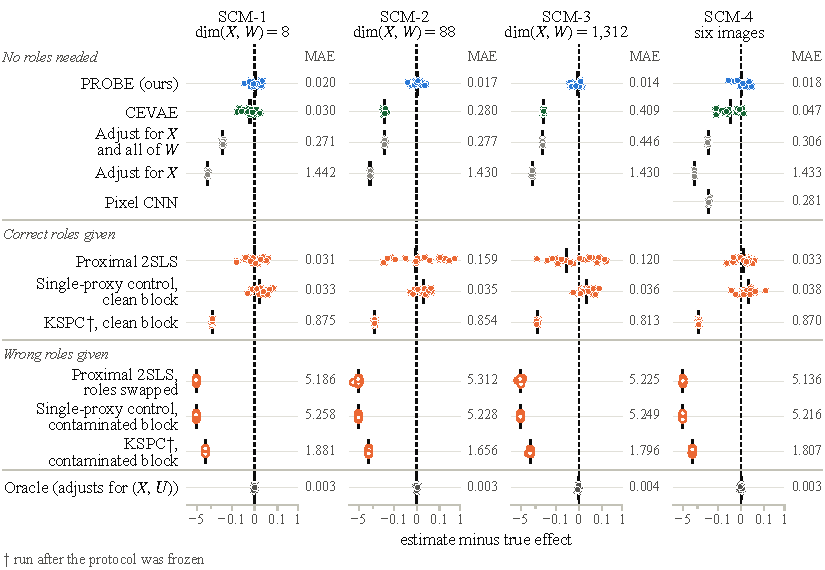
\includegraphics[width=\linewidth]{probe-estimates-v3.pdf}
\caption[Detailed errors in the synthetic settings.]{Detailed version of the left of Fig.~\ref{fig:experiments} for the original $20$ data sets per setting, with every method on its own row. KSPC ($\dagger$) was run after the protocol was frozen.}
\label{fig:synthetic-detail}
\end{figure}

\begin{figure}[t]
\centering
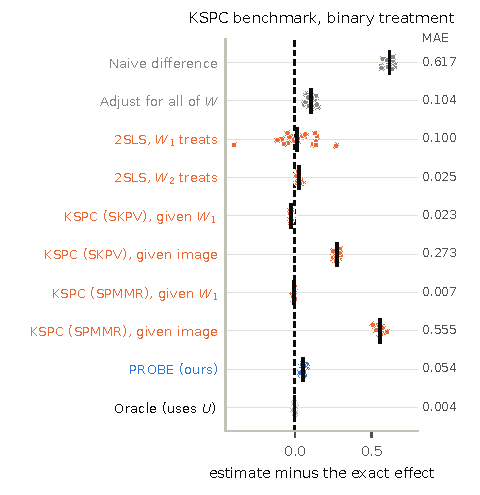
\includegraphics[width=0.55\linewidth]{probe-kspc.pdf}
\caption[Kernel single-proxy benchmark.]{Kernel single-proxy benchmark of \citet{xu2025kernel} with a binary treatment; the effect is exactly $1$. Estimates minus the effect over $20$ replicates, with the MAE on the right.}
\label{fig:appendix-kspc}
\end{figure}

Fig.~\ref{fig:synthetic-detail} gives the detailed comparison. PROBE answers every one of the $80$ original data sets, with mean absolute error between $0.014$ and $0.020$ and 90th percentile error between $0.033$ and $0.046$. Its prespecified one-sided paired bound on the excess over the oracle ranges from $0.015$ to $0.023$. The two ways of using the proxy without an audit both fail: adjustment for $X$ and the entire raw proxy has mean estimate between $0.55$ and $0.73$ because it absorbs the treatment-only coordinate, and in SCM-4 a convolutional network that reads every pixel and never tests balance has mean estimate $0.72$. The paired bound against that pixel network is $-0.25$.

The prespecified-block contrast isolates identification from search, as Thm.~\ref{thm:exact-proxy-identification} requires. Holding out the clean block $W_1$ and balancing it gives $0.998$, $0.987$, $0.980$ and $1.000$ in the four settings. Holding out the contaminated block $W_4$ gives $0.660$, $0.656$, $0.616$ and $0.667$, and the balance screen retains that split in $79$ of the $80$ original data sets and $396$ of all $400$, because $W_4$ really can be balanced. Holding out $W_5$ gives about $0.29$ and is rejected in all $80$ original data sets and all $400$, since no representation balances a block that carries the treatment-only cause. Balance is observable, and on its own it is not enough.

Aggregation repairs the one failure that balance leaves. Thm.~\ref{thm:unknown-valid-block-identification} and Cor.~\ref{cor:target-majority-median} predict that the valid splits outvote $W_4$ when they form a majority, and they do: averaging over the retained splits is dragged to $0.963$, $0.956$, $0.945$ and $0.959$, the plain median of the retained splits already recovers most of that at $1.002$, $0.998$, $0.991$ and $0.997$, and the median of the largest agreeing component that PROBE returns reaches $1.005$, $1.003$, $0.993$ and $1.001$. The screen has true positive rate between $0.986$ and $1.000$ and false positive rate between $0.041$ and $0.046$, every returned component is pure, and every data set returns a unique largest component.

The two bounds of Thm.~\ref{cor:representation-causal} and Thm.~\ref{thm:conditional-aipw-error} are visible separately. For a single split in SCM-1 to SCM-3, the population effect of the learned representation sits a median of $0.042$ to $0.046$ from $\tau$, with 90th percentile $0.103$ to $0.110$, and the realised error of that one split has median $0.051$ to $0.059$. Aggregating the retained splits cuts this to the $0.014$ to $0.020$ reported above, so the combination step, not a single well-behaved representation, carries the accuracy. The same separation shows up in the intervals. A nominal $95\%$ interval around one split, built from the estimate's own standard error, covers $\tau_{\widehat Z}$ at $0.950$, $0.957$ and $0.936$ in SCM-1 to SCM-3, which is the nominal rate, and covers $\tau$ at $0.836$, $0.857$, $0.879$ and $0.807$. The shortfall is the representation gap, which no interval built from sampling variation can contain; Fig.~\ref{fig:appendix-coverage} shows it per data set.

Two boundaries limit what these results show. The image setting hands PROBE numbers produced by a reader that was trained with orientation labels on an auxiliary image bank, disjoint from the causal data; that reader made no level error in $14{,}400{,}000$ reads of all $100$ data sets, so SCM-4 tests the pipeline under an image proxy rather than the discovery of a representation from raw pixels. The second boundary is the one the $W_4$ contrast exposes: the screen certifies balance and cannot certify the outcome-relevant condition that Assumption~\ref{ass:outcome-relevant-completeness} adds.

\begin{table}[t]
\caption{Sealed confirmations. Each row is $20$ independently generated data sets at $n=24{,}000$.}
\label{tab:verified-results}
\centering
\footnotesize
\begin{tabular}{llrrrl}
\toprule
Setting & \shortstack[l]{\\What the learner sees} & Mean error & p90 & Oracle gap & Status \\
\midrule
SCM-1 & $8$ coordinates & 0.020 & 0.033 & 0.022 & 12/12 gates \\
SCM-2 & $88$ coordinates & 0.017 & 0.037 & 0.019 & 12/12 gates \\
SCM-3 & $1{,}312$ coordinates & 0.014 & 0.035 & 0.015 & 12/12 gates \\
SCM-4 & six $64\times64$ images & 0.018 & 0.046 & 0.023 & 13/13 gates, amended \\
\bottomrule
\end{tabular}
\end{table}

The SCM-4 row carries a correction that we report rather than hide. Two of its $20$ data sets reached the wall-clock cap while three tasks shared one GPU, so the pixel-network comparator recorded no value there and the sealed summary returned FAIL on the completeness gate and on the comparison that depends on it. Those two comparator runs were repeated alone under the sealed configuration and the sealed seeds, every other number was left untouched, and the amended summary passes all $13$ gates.

\begin{figure}[t]
\centering
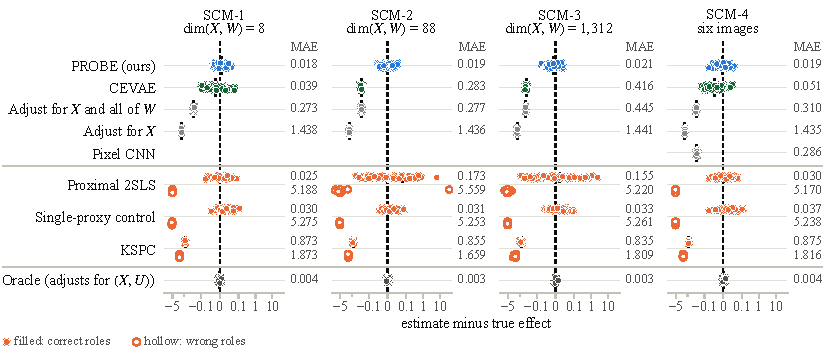
\includegraphics[width=\linewidth]{probe-synthetic-v5-found.pdf}
\caption[Detailed synthetic results.]{Detailed version of the left of Fig.~\ref{fig:experiments} over all $100$ data sets per setting, with the MAE of each method on the right; for methods that need proxy roles, the upper number is for the correct roles. PROBE finds the blocks from $W$ (Appendix~\ref{sec:appendix-block-discovery}) except in SCM-4, where they are given.}
\label{fig:appendix-synthetic}
\end{figure}

\begin{figure}[t]
\centering
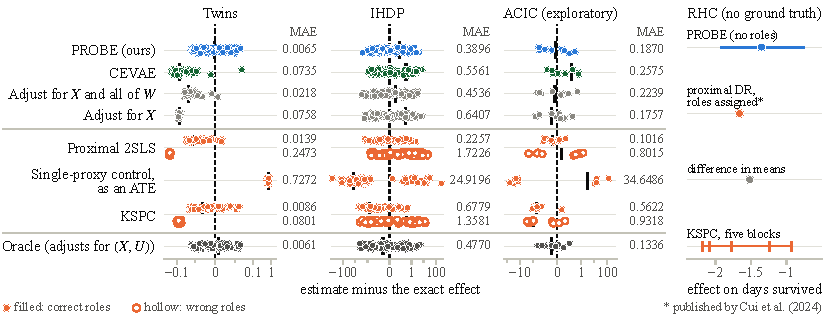
\includegraphics[width=\linewidth]{probe-realdata-v5-found.pdf}
\caption[Detailed semi-synthetic and RHC results.]{Detailed version of the right of Fig.~\ref{fig:experiments} over $100$ Twins, $88$ IHDP, and $9$ ACIC data sets, with the MAE of each method, and the RHC estimates, where no true effect is known; PROBE's estimate carries its resampled $95\%$ interval, and * marks estimates published by \citet{cui2024semiparametric}. PROBE finds the blocks from $W$, including the ten RHC measurements (Appendix~\ref{sec:appendix-block-discovery}).}
\label{fig:appendix-realdata}
\end{figure}

\subsection{Chest X-ray analysis}
\label{sec:appendix-single-image}

\paragraph{Data and hidden confounder.} The images are the $64\times64$ release of PneumoniaMNIST in MedMNIST+ \citep{yang2023medmnist}, built from the pediatric chest X-ray collection of \citet{kermany2018identifying} (CC BY 4.0): $5{,}856$ images, $1{,}583$ normal and $4{,}273$ with pneumonia, with the official training, validation, and test parts pooled. The hidden confounder $U$ is the standardised logit of a small convolutional classifier of the pneumonia label, fitted on one half of the images and applied to the other half and vice versa (six epochs; cross-fitted AUC $0.983$). The binary label itself is not used as $U$, because the image carries only part of it: a linear probe on whole-image features explains $66\%$ of its variance, so no adjustment that uses the image could recover the effect. The logit is an image-determined severity, and the representation below recovers $91\%$ of its variance. Treatment and outcome follow $P(A=1\mid U)=0.1+0.8\,\Phi(1.5U)$ and $Y=A+U+\varepsilon$ with $\varepsilon\sim N(0,1)$, so $\tau=1$, except in the mediator scenario below. Each of the $50$ replicates of a scenario redraws $A$, $Y$, the noise, and the overlays; the images are fixed. The $50$ replicates were generated with new seeds after an exploratory phase of ten replicates per scenario, on which the rule below was fixed.

\paragraph{Blocks and scenarios.} In pixel coordinates (row, column; zero-based, inclusive), $W_1$ is rows $8$ to $30$ and columns $4$ to $27$, $W_2$ rows $33$ to $55$ and columns $4$ to $27$, $W_3$ rows $8$ to $30$ and columns $36$ to $59$, $W_4$ rows $33$ to $55$ and columns $36$ to $59$, and $W_5$ rows $0$ to $63$ and columns $29$ to $34$. Blocks are separated by at least two pixels, and every overlay is drawn only on the pixels of its block. A \emph{device} is a vertical line of intensity $+0.35$ at rows $4$ to $44$ and columns $31$ to $32$ of $W_5$, drawn with probability $0.9$ when $A=1$ and $0.1$ when $A=0$; the footprint in a lung block draws the same line at rows $36$ to $52$ and columns $14$ to $15$ of $W_2$. A \emph{response mark} is a Gaussian spot of standard deviation two pixels with amplitude $0.25$ times the standardised value of $U-\kappa A+0.5\nu$, $\nu\sim N(0,1)$, clipped to $[-2.5,2.5]$, with $\kappa=1.5$ unless stated; it is centred at row $20$, column $31.5$ in $W_5$, at row $44$, column $15.5$ in $W_2$, and at rows $19$ and $44$ and columns $15.5$ and $47.5$ in the four quadrants. The scenarios are: clean; device in $W_5$; device line in $W_2$; response mark in $W_5$; mediator, in which $M=A+0.5\nu$ darkens the position of the mark in $W_5$ by $0.25$ times its standardised value and $Y=0.5A+0.5M+U+\varepsilon$, so that the total effect is still $1$ and adjustment for the mark targets the direct effect $0.5$; the response mark in $W_2$ and $W_5$, drawn from one value of $U-1.5A+0.5\nu$; the response mark in all five blocks; a device collider, the line in $W_5$ drawn with probability $\operatorname{expit}(-2+2A+1.5U)$ ($11\%$ of untreated and $67\%$ of treated units); the device in $W_5$ together with the response mark in $W_2$; a near-deterministic device, the line in $W_5$ drawn with probability $0.98$ when $A=1$ and $0.02$ when $A=0$; and the imprint sweep, the response mark in $W_5$ with $\kappa\in\{0,0.5,1,2,3\}$.

\paragraph{Block-additive representation.} The features of block $k$ come from a network that sees the image with only block $k$ visible, the other pixels set to zero and a visibility channel appended. The network has the convolutional trunk of the synthetic image experiments and a head that predicts $A$ by the logistic loss and the standardised $Y$ by the squared loss from the block alone; it is trained for six epochs on one half of the units and applied to the other half and vice versa, so that no unit's features come from a network that saw that unit's treatment or outcome. Its pooled trunk output ($128$ numbers) is reduced to $16$ principal components fitted on all rows without labels, and the five blocks are concatenated to $80$ features; hiding a block removes exactly its $16$ features. The cross-validated $R^2$ of $U$ on the $80$ features is $0.91$ in every scenario. An unsupervised masked autoencoder \citep{he2022masked} in place of the supervised trunk gave $R^2=0.875$ and a higher floor in the exploratory runs and is not used here. Whole-image features are not block-additive: hiding a block changes the embedding of the remaining pixels, which confounds the information cost of hiding a block with a change of the remaining representation.

\paragraph{Audit and estimation.} For block $j$, the retained representation $Z_{-j}$ stacks the features of the other blocks, and the held-out block $T_j$ is the pixel vector of block $j$ reduced by the per-block principal component rule of the sealed code. The screen of Appendix~\ref{sec:appendix-experiments} is applied unchanged on each of the four rotations, and the gap and its standard error are pooled over rotations. The rule flags the block with the largest gap when that gap exceeds the median gap of the audited blocks by more than two standard errors and exceeds an absolute floor of $0.005$; the flagged block is hidden, the remaining blocks are audited again, and the step repeats at most once more, so that at most two blocks are hidden. The absolute thresholds of the synthetic settings do not transfer, because the noise level of the gap depends on the $80$-dimensional representation, for the same reason that led to the noise-scaled rule of Appendix~\ref{sec:appendix-benchmarks}. The one-pass rule of the exploratory phase, which flags every block whose gap exceeds the median by more than two standard errors without a floor or a second audit, is reported alongside. The estimate is the sealed AIPW on the remaining blocks; adjustment for the whole image, the pixel CNN of the main text, uses all $80$ features in the same AIPW, and the oracle adjusts for $U$. On clean images the five gaps lie between $-0.0004$ and $0.0004$ with standard errors near $0.001$; a block that carries a mark has a gap of $0.036$ to $0.21$.

\paragraph{Results.} Table~\ref{tab:single-image-appendix} gives all scenarios. Under the sequential rule the hidden blocks are exactly the blocks that carry the mark in all $50$ replicates of the response, mediator, two-block, device-and-response, and near-deterministic-device scenarios, in $49$ of the lung-footprint replicates, and nothing is hidden in any clean replicate. The one-pass rule differs in two ways: it flags a clean block in addition to the marked one in up to $13$ replicates per scenario, because the mark left in $Z_{-j}$ raises the gaps of the clean blocks from about $0.001$ to about $0.004$, and it misses the second block of the two-block response in $45$ replicates, because given $W_5$ the mark in $W_2$ repeats information the representation already holds, so its gap is small until $W_5$ is hidden. A device alone, drawn by $A$ and noise, does not change the estimate whether it is hidden or kept, as Prop.~\ref{prop:single-image-decomposition}(c) states; the near-deterministic device raises the MAE of the pixel CNN to $0.16$, against $0.14$ for the device in $W_5$, without a visible bias, and hiding it removes the increase. Two scenarios show where exclusion stops helping. When the response mark is drawn in every block, the five gaps are similar ($0.0005$ to $0.008$), the median is itself a marked block's gap, and hiding the block with the largest gap only loses information ($1.44$ against $1.39$). The device collider is a block whose two causes act in the same direction, so conditioning on it induces a negative association between $A$ and $U$ that offsets part of the positive residual confounding; the screen flags it because it carries $A$, and hiding it costs $0.04$. Exclusion therefore helps when content that $A$ and $U$ jointly cause, or that $A$ passes on to $Y$, is confined to few blocks and moves the estimate away from $\tau$, and the main text reports the scenarios of each kind.

\begin{table}[t]
\caption{Chest X-ray analysis, all scenarios (hand-drawn blocks, supervised encoder, $50$ replicates, true effect $1$): mean estimate, with the MAE in parentheses. The last column counts the replicates in which the sequential rule hides exactly the blocks that carry the mark; in the clean scenario, the replicates in which it hides nothing. The difference in means is between $2.10$ and $2.12$ in every scenario.}
\label{tab:single-image-appendix}
\centering
\footnotesize
\begin{tabular}{lccccc}
\toprule
Scenario & Pixel CNN & PROBE, one pass & PROBE, sequential & Oracle & Exact \\
\midrule
Clean & 1.132 (0.132) & 1.135 (0.135) & 1.132 (0.132) & 0.999 & 50 \\
Device in $W_5$ & 1.137 (0.139) & 1.129 (0.129) & 1.128 (0.128) & 0.998 & 50 \\
Device line in $W_2$ & 1.158 (0.158) & 1.163 (0.163) & 1.161 (0.161) & 1.006 & 49 \\
Response in $W_5$ & 1.268 (0.268) & 1.150 (0.150) & 1.138 (0.138) & 1.003 & 50 \\
Mediator in $W_5$ & 0.740 (0.260) & 1.152 (0.152) & 1.149 (0.149) & 1.016 & 50 \\
Response in $W_2$ and $W_5$ & 1.327 (0.327) & 1.295 (0.295) & 1.171 (0.171) & 1.001 & 50 \\
Device in $W_5$ and response in $W_2$ & 1.291 (0.291) & 1.164 (0.164) & 1.164 (0.164) & 0.993 & 50 \\
Response in every block & 1.390 (0.390) & 1.430 (0.430) & 1.436 (0.436) & 0.992 & -- \\
Device collider in $W_5$ & 1.088 (0.090) & 1.129 (0.129) & 1.130 (0.130) & 0.995 & 48 \\
Near-deterministic device in $W_5$ & 1.148 (0.155) & 1.128 (0.128) & 1.126 (0.126) & 0.994 & 50 \\
\bottomrule
\end{tabular}
\end{table}

\paragraph{Imprint sweep.} Fig.~\ref{fig:single-image} (right) repeats the response scenario with $\kappa\in\{0,0.5,1,1.5,2,3\}$. The MAE of the pixel CNN is $0.10$, $0.19$, $0.24$, $0.27$, $0.33$, and $0.57$, and that of PROBE $0.10$, $0.14$, $0.13$, $0.14$, $0.12$, and $0.14$. At $\kappa=0$ the mark is a function of $U$ and noise, the gap of $W_5$ is $0.0008$, nothing is hidden, and the extra information about $U$ lowers both errors below the clean case ($R^2=0.93$). At $\kappa=0.5$ the gap is $0.009$ and $W_5$ is hidden in $44$ replicates; from $\kappa=1$ on it is hidden in all $50$.

\paragraph{Automatic block layouts.} The five blocks above were drawn by hand from anatomy. Table~\ref{tab:single-image-layouts} repeats the main scenarios with a $4\times4$ grid of $16$-pixel cells, eight principal components per cell, the same encoder, the same rule with at most three cells hidden, and the same replicates. The grid covers the whole image but carries no more of $U$ ($R^2=0.91$) and gives a similar error on clean images ($0.12$ against $0.13$). A mark straddles two cells, and the grid hides both only when each has a gap of its own: under the response it does so in all replicates and the error matches the hand-drawn blocks, whereas under the mediator both cells are hidden in $20$ of $50$ replicates and the MAE stays at $0.22$. The hand-drawn layout was therefore kept, by a rule fixed before these replicates were run. In the exploratory phase, with the masked autoencoder, grids of $3\times3$ and $4\times4$ cells had given the same or a smaller error than the hand-drawn blocks under a treatment response.

\begin{table}[t]
\caption{Chest X-ray analysis with a $4\times4$ grid in place of the hand-drawn blocks (supervised encoder, $50$ replicates, true effect $1$): mean estimate of adjustment for all cells and of PROBE, with the MAE in parentheses.}
\label{tab:single-image-layouts}
\centering
\footnotesize
\begin{tabular}{lcccc}
\toprule
 & \multicolumn{2}{c}{Hand-drawn blocks} & \multicolumn{2}{c}{$4\times4$ grid} \\
\cmidrule(lr){2-3}\cmidrule(lr){4-5}
Scenario & Pixel CNN & PROBE & All cells & PROBE \\
\midrule
Clean & 1.132 (0.132) & 1.132 (0.132) & 1.119 (0.120) & 1.119 (0.120) \\
Response in $W_5$ & 1.268 (0.268) & 1.138 (0.138) & 1.325 (0.325) & 1.127 (0.128) \\
Mediator in $W_5$ & 0.740 (0.260) & 1.149 (0.149) & 0.714 (0.286) & 0.871 (0.225) \\
Response in $W_2$ and $W_5$ & 1.327 (0.327) & 1.171 (0.171) & 1.359 (0.359) & 1.289 (0.289) \\
Response in every block & 1.390 (0.390) & 1.436 (0.436) & 1.407 (0.407) & 1.421 (0.421) \\
Device collider in $W_5$ & 1.088 (0.090) & 1.130 (0.130) & 1.074 (0.081) & 1.074 (0.081) \\
\bottomrule
\end{tabular}
\end{table}

\paragraph{Resolution.} Doubling the resolution does not lower the floor. With the $128\times128$ release of the same images, the masks and overlays scaled by two, the same encoder, and the sequential rule, we ran the clean, device-in-$W_5$, device-line-in-$W_2$, and response scenarios with $10$ data sets each on new seeds. The $R^2$ of $U$ is $0.907$ ($0.900$ to $0.911$), as at $64$ pixels. On clean images the pixel CNN and PROBE both give $1.104$ (MAE $0.107$), and under the treatment response the pixel CNN gives $1.250$ ($0.250$) and PROBE $1.140$ ($0.140$), against $1.132$ ($0.132$), $1.268$ ($0.268$), and $1.138$ ($0.138$) at $64$ pixels in Table~\ref{tab:single-image-appendix}; each difference is about one standard error of a mean over ten data sets ($0.01$ to $0.02$) or less. PROBE hides nothing in any clean data set and exactly the marked block in all $30$ marked data sets. The hidden $U$ is computed from the $64$-pixel images, so the higher resolution adds no information about it; the floor is set by the encoder and by the pixels that the blocks cover, not by the number of pixels.

\paragraph{What this experiment does and does not show.} The overlays are synthetic and the data set is one. In the scenarios where exclusion helps, the treatment-dependent content sits in one or two regions that carry little of $U$; a treatment response in the lungs themselves, where most of $U$ is, falls under the every-block scenario, in which exclusion cannot help. Exploratory runs that preceded this design are kept in the repository and bound the claim: on a lung phantom without treatment-dependent content, and on the clean X-rays, adjusting for the whole image was as accurate as PROBE or more accurate, because holding out a block costs information and there was nothing to exclude; learning the representation from pixels with the balance objective alone, by a rank-two linear map or by fine-tuning a convolutional network, was less accurate than the block-additive encoders; and the gap that remains between every image-based method and the oracle is the part of $U$ that the image representation does not carry, which Prop.~\ref{prop:single-image-decomposition} shows no choice of blocks can remove.

\subsection{Semi-synthetic benchmarks}
\label{sec:appendix-benchmarks}

Twins \citep{louizos2017causal}, IHDP \citep{hill2011bayesian}, and ACIC 2016 \citep{dorie2019automated} keep their covariates and both potential outcomes, so the effect is known exactly. In each, one covariate is hidden as $U$ (gestational age in Twins, the sixth of the $25$ IHDP covariates, and $x_{44}$ in ACIC), and the five proxy blocks and the treatment are generated from it by one fixed recipe. The blocks follow the proxy mechanism of SCM-1 with a generated standard normal treatment-only cause $I$, and the treatment follows $P(A=1\mid U,I,X)=0.1+0.8\,\Phi(1.5U+2.0I+w^\top\tilde X)$, where $U$ is standardised, $\tilde X$ is the standardised $X$, and $w\sim N(0,0.1^2I)$ is drawn once. Twins has $n=11{,}984$ and $42$ covariates, IHDP $n=747$ and $24$, and ACIC $n=4{,}802$ and $78$. The original runs use Twins replicates $11$ to $20$, IHDP replicates $12$ to $21$, and ACIC realizations $2$ to $10$. The comparators take the proxy roles of Appendix~\ref{sec:appendix-synthetic-results}; single-proxy control is run once, as an ATE estimator with the clean block $W_1$.

The sealed thresholds of SCM-1 to SCM-4 do not transfer to these data sets, because the noise level of the screen statistic changes with the numbers of rows and covariates. The screen therefore uses a noise-scaled threshold: instead of requiring a pass in all four rotations, it pools them, taking their mean gap and its standard error, and it retains a split when $\max(\mathrm{gap},0)+z\,\mathrm{SE}$ is at most the median of $z\,\mathrm{SE}$ over the thirty splits of the same data set. This rule was adopted after the pre-registered RHC analysis and the RHC-planted, ACIC, and earlier IHDP analyses with the sealed threshold returned no estimate. It was frozen before Twins replicates $11$ to $20$ and IHDP replicates $12$ to $21$ were generated, so these two studies are prospective tests; it was chosen after seeing ACIC realizations $2$ to $10$, so the ACIC results are exploratory.

\paragraph{RHC study.}\label{sec:appendix-rhc} The RHC study \citep{connors1996effectiveness} has $5{,}735$ critically ill patients, days survived within $30$ as the outcome, and ten physiological measurements grouped into five proxy blocks, as analyzed by \citet{cui2024semiparametric}; no true effect is known. The blocks are, in order, the PaO$_2$/FiO$_2$ ratio and PaCO$_2$, pH and hematocrit, white cell count and albumin, bilirubin and creatinine, and sodium and potassium, and the comparators are the difference in means, the proximal estimate that \citet{cui2024semiparametric} obtain by assigning roles to $W_1$ and $W_2$, and KSPC given each block in turn. PROBE is not given this grouping and finds its own blocks from the ten measurements (Appendix~\ref{sec:appendix-block-discovery}). The interval around PROBE's RHC estimate in Fig.~\ref{fig:appendix-realdata} gives the sampling spread of the median of the largest agreeing group over $20{,}000$ draws, holding the retained splits and the linking radius at their observed values, so it omits the uncertainty of the screen. PROBE's interval contains the proximal estimate that \citet{cui2024semiparametric} obtain by assigning the roles, while KSPC's estimate changes with the block it is given (Fig.~\ref{fig:appendix-realdata}).

Table~\ref{tab:benchmarks} gives the MAE on the original replicates. On IHDP, ten replicates do not resolve the gap between PROBE and CEVAE: the error ratio is $1.67$, with a $90\%$ paired-bootstrap interval from $0.78$ to $2.78$.

\begin{table}[t]
\caption{Mean absolute error on the original replicates in three semi-synthetic studies with known effects; ACIC is exploratory. Proximal 2SLS, single-proxy control, and KSPC require proxy roles; KSPC ($\dagger$) was run after the protocol was frozen. Bold marks the smallest error among the methods other than the oracle.}
\label{tab:benchmarks}
\centering
\footnotesize
\begin{tabular}{lrrr}
\toprule
Method & Twins & IHDP & ACIC \\
\midrule
PROBE (ours) & \textbf{0.0077} & 0.3054 & 0.2025 \\
CEVAE & 0.0894 & \textbf{0.1828} & 0.2575 \\
Adjust for $X$ and all of $W$ & 0.0207 & 0.3927 & 0.2239 \\
Adjust for $X$ & 0.0749 & 0.7221 & 0.1757 \\
Proximal 2SLS, roles given & 0.0156 & 0.2328 & \textbf{0.1016} \\
Proximal 2SLS, roles swapped & 0.2453 & 1.5856 & 0.8015 \\
Single-proxy control, as an ATE & 0.7318 & 5.9838 & 34.6486 \\
KSPC$^\dagger$, clean block & 0.0099 & 0.6214 & 0.5622 \\
KSPC$^\dagger$, contaminated block & 0.0815 & 1.2499 & 0.9318 \\
\midrule
Oracle (adjusts for $(X,U)$) & 0.0074 & 0.4868 & 0.1336 \\
\bottomrule
\end{tabular}
\end{table}

\subsection{Protocol discipline}

One generated data set is one replicate; splits, rows, rotations, and restarts are not. Seeds overlap across the synthetic settings: SCM-1 replicates $10$ to $19$ share seeds with SCM-2 replicates $0$ to $9$, and SCM-2 replicates $10$ to $19$ with SCM-3 replicates $0$ to $9$, so comparisons across those settings are not independent. Paired methods share data, sample roles, and nuisance budgets. For SCM-1 to SCM-4 the screen threshold is fixed before the confirmation data are generated, and Appendix~\ref{sec:appendix-benchmarks} gives the rule and its history for the other data sets. The threshold remains a screen rather than proof of causal validity. No-return outcomes stay in the return-rate denominator, failed sealed runs stay in the record, and this appendix documents exclusions, replacements, and the representation family the search ranges over.

\subsection{Evidence boundaries}

 The empirical gates are performance criteria, not proofs of completeness, stability, or the population plurality condition.

\subsection{Additional figures}

Fig.~\ref{fig:appendix-aggregation} shows the three aggregation rules on the sealed confirmations, Fig.~\ref{fig:appendix-coverage} shows the interval coverage of one split, and Fig.~\ref{fig:appendix-learned} separates the representation and estimation parts of the error.

The interval in Fig.~\ref{fig:appendix-coverage} is the AIPW estimate of one split plus or minus $1.96$ times its own standard error, and that standard error is computed from the score cross-product the sealed run already stored, so the figure refits nothing. It covers what the learned representation targets at the nominal rate and covers $\tau$ less often, by the amount of the representation gap. An interval built from sampling variation cannot contain that gap, which is why Thm.~\ref{cor:representation-causal} bounds it separately from Thm.~\ref{thm:conditional-aipw-error}.

\begin{figure}[t]
\centering
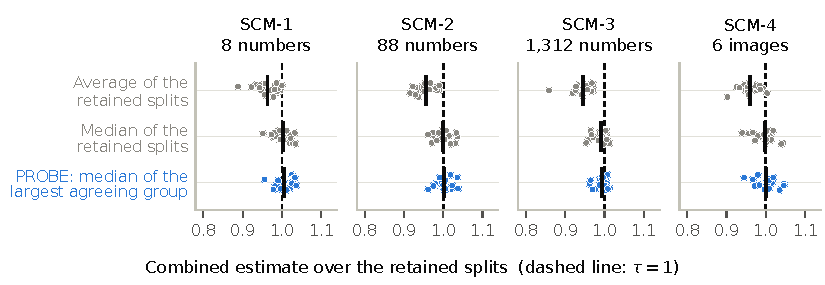
\includegraphics[width=\linewidth]{probe-aggregation.pdf}
\caption[Aggregation rules.]{Three ways to combine the retained splits. Averaging is pulled away from $\tau$ by the balanced but invalid split; the median of the largest agreeing group is not.}
\label{fig:appendix-aggregation}
\end{figure}

\begin{figure}[t]
\centering
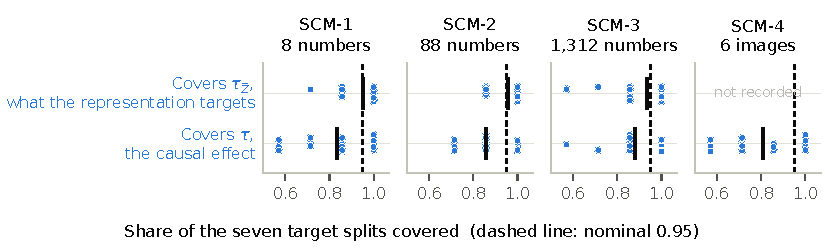
\includegraphics[width=\linewidth]{probe-coverage.pdf}
\caption[Interval coverage.]{Coverage of a nominal $95\%$ interval around one split, one dot per data set. The interval covers the population effect of the learned representation at the nominal rate and covers $\tau$ less often, by the representation gap.}
\label{fig:appendix-coverage}
\end{figure}

\begin{figure}[t]
\centering
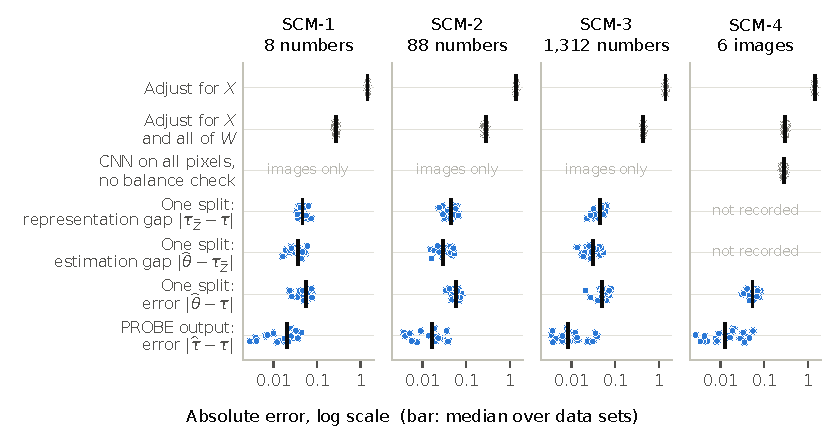
\includegraphics[width=\linewidth]{probe-learned.pdf}
\caption[Absolute errors of one split and of aggregation.]{Absolute errors on a log scale. For one split the representation gap $|\tau_{\widehat Z}-\tau|$ is the population effect of the learned representation, which is exact for the linear representations of SCM-1 to SCM-3 and is not recorded for SCM-4. Aggregation reduces the error of a single split by roughly a factor of three.}
\label{fig:appendix-learned}
\end{figure}

\FloatBarrier

